\documentclass[a4paper, 11pt]{report}
\usepackage{../../preamble}
\usepackage{ amssymb }
\usepackage{tabularx}
\DeclareMathOperator{\Hessian}{Hess}
\usepackage{graphicx}

\newcommand{\rotvert}{\rotatebox[origin=c]{90}{$\vert$}}

\renewcommand{\clearpage}{}
\renewcommand{\cleardoublepage}{}
\setlength{\parindent}{0pt}

\begin{document}

\doctype{Homework}
\coursetitle{Probabilistic Graphical Models}
\semester{MVA Fall 2019}
\instructor{Pierre Latouche}
\student{Antoine Moulin, Marie Heurtevent}
\worknumber{2}
\workdate{December 31}

\maketitle

\chapter{Classification: K-means, and the EM algorithm}


Consider a mixture model, with $K$ components, where datapoints $X_i$, $i = 1, . . . , n$ have a probability $p_k$ to be in component $k$: $P(Z_i = k) = p_k$, and, conditional on $Z_i = k$, $X_i \sim \mathcal{N}(\mu_k,D_k)$, a multivariate Gaussian distribution with mean $\mu_k$, and diagonal (not full) covariance matrix $D_k$.

\begin{enumerate}
    \item Derive the expressions of the parameter $\theta_k = (p_k, \mu_k, D_k)$ at each iteration of the corresponding EM algorithm.
        \vspace{0.3cm} \\
        \textbf{Solution.}\\
        First, let's compute the likelihood of the problem at the t-th iteration. 
        
        \begin{align*}
            \ell_t &= \log p_\theta(X,Z) \\
            &= \sum_{i=1}^{n} \log p_\theta(X_i,Z_i)\\
            &= \sum_{i=1}^{n} \log p_\theta(Z_i) + \sum_{i=1}^{n} \log p_\theta(X_i | Z_i)\\
            \ell_t &= \sum_{i=1}^{n} \sum_{j=1}^{K} z_i^j \log p_j + \sum_{i=1}^{n} \sum_{j=1}^{K} z_i^j \log \mathcal{N}(X_i | \mu_{j,t}, D_{j,t})\\
        \end{align*}
    
    with $z_i^j =& \left\{
                        \begin{array}{ll}
                            1 \mbox{ if } z_i = j \\
                            0 \mbox{ otherwise}
                        \end{array}
                    \right.$ 
    and $\mathcal{N}(X_i | \mu, D) = \frac{1}{(2 \pi)^{\frac{d}{2}}|D|^{\frac{1}{2}}} \exp{\{-\frac{1}{2}(x_i - \mu)^TD^{-1}(x_i-\mu)\}}$. \\
    
    \textbf{During the E-step,} we will write the expectation of the complete likelihood at step $t$ with respect to the conditional distribution of $Z | X$. \\
    Since, all terms of the sum except for $z_i^j$ are constant with regards to $Z | X$, we need to compute $\mathbb{E}_{(Z |X)}(z_i^j)$.
    
    \begin{align*}
        \mathbb{E}_{(Z |X)}(z_i^j) =& p_{\theta_t}(z_i = j | x_i) \\
        =& \frac{p_{\theta_t}(z_i = j, x_i)}{p_{\theta_t}(x_i)} \\
        =& \frac{p_{\theta_t}(z_i = j)p_{\theta_t}(x_i | z_i = j)}{p_{\theta_t}(x_i)} \\
        =& \frac{p_j \mathcal{N}(x_i | \mu_j, D_j)}{\sum_{j'} p_{j'} \mathcal{N}(x_i | \mu_{j'}, D_{j'})} \\
        :=& \tau_i^j(\theta_t)
    \end{align*}
    Since the value of $\theta_t$ will be fixed during the M-step, we can drop the dependence on $\theta_t$ and write $\tau_i^j$. \\
    Hence,
    \begin{align*}
        \mathbb{E}_{(Z |X)}(l_t) &= \sum_{i=1}^{n} \sum_{j=1}^{K} \tau_i^j \log p_j + \sum_{i=1}^{n} \sum_{j=1}^{K} \tau_i^j \log \mathcal{N}(X_i | \mu_{j,t}, D_{j,t}) \\
        \mathbb{E}_{(Z |X)}(l_t) &= \sum_{i=1}^{n} \sum_{j=1}^{K} \tau_i^j \log p_j + \sum_{i=1}^{n} \sum_{j=1}^{K} \tau_i^j \left[ \log\left(\frac{1}{(2 \pi)^{\frac{d}{2}}}\right) + \log\left(\frac{1}{|D_{j,t}|^{\frac{1}{2}}}\right)-\frac{1}{2}(x_i - \mu_{j,t})^TD_{j,t}^{-1}(x_i-\mu_{j,t}) \right]\\
    \end{align*}
    
    
    \textbf{During the M-step,} we will maximise the previous expectation with respect to $\theta_t = (p_t, \mu_t, D_t)$.\\
    The expectation is split into two independent terms so we can start by first maximizing with regards to $p_t$:
    \begin{flalign*}
        & \max_{p} \sum_{i=1}^{n} \sum_{j=1}^{K} \tau_i^j \log p_j &
    \end{flalign*}
    which gives us:
    \begin{flalign*}
        p_{j,t+1} &= \frac{\sum_{i=1}^{n} \tau_i^j}{\sum_{i=1}^{n} \sum_{j'=1}^{K} \tau_i^{j'}} & \\
        p_{j,t+1} &= \frac{1}{n}\sum_{i=1}^{n} \tau_i^j &
    \end{flalign*}
    because $\sum_{j'=1}^{K} \tau_i^{j'} = \sum_{j'=1}^{K} p_{\theta} (z_i = j' | x_i) = 1$. \\
    
    We can now maximize the right term of the sum with regards to $\mu_t$ and $D_t$, which leaves us with:
    \begin{flalign*}
        \mu_{j,t+1} &= \frac{\sum_{i=1}^{n} \tau_i^j x_i}{\sum_{i=1}^{n} \tau_i^j} & \\
        D_{j,t+1} &= \frac{\sum_{i=1}^{n} \tau_i^j \left(x_i - \mu_{j,t+1} \right) \left( x_i - \mu_{j,t+1} \right)^T}{\sum_{i=1}^{n} \tau_i^j} &
    \end{flalign*}
    
    We can name $w_j^t := \sum_{i=1}^{n} \tau_i^j(\theta_t)$.
    
    
    Hence, the updated expressions of the parameters at each iteration are 

    \begin{equation*}
        \boxed{\begin{aligned}
        p_{j,t+1} &= \frac{1}{n} w_j^t \\
        \mu_{j,t+1} &= \frac{1}{w_j^t} \sum_{i=1}^{n} \tau_i^j x_i \\
        D_{j,t+1} &= \frac{1}{w_j^t} Diag(x_i - \mu_{t+1})^{2}
        \end{aligned}}
    \end{equation*}
    
        
    \item What may be the advantage of such a model, compared to the more standard Gaussian mixture model, where covariance matrices are full? 
    
        \textbf{Solution.}\\
        In general, when the covariance matrices are full, there are $O \left( K\frac{d(d+1)}{2} \right)$ parameters. In this case, there are much fewer parameters : $O \left(Kd\right)$. \\
        For datasets that feature relatively independant features conditionally on the latent class, this approximation is quite valid with very similar performances, all the while retaining much fewer parameters.
        
    \item Implement the algorithm, and compare the results with: 
            \begin{itemize}
                \item K-means
                \item EM for a standard Gaussian mixture (full covariance)
            \end{itemize}
    for the IRIS data set, and $K = 2, 3, 4$. 
    
        \textbf{Solution.}\\
        \begin{figure}
            \centering
            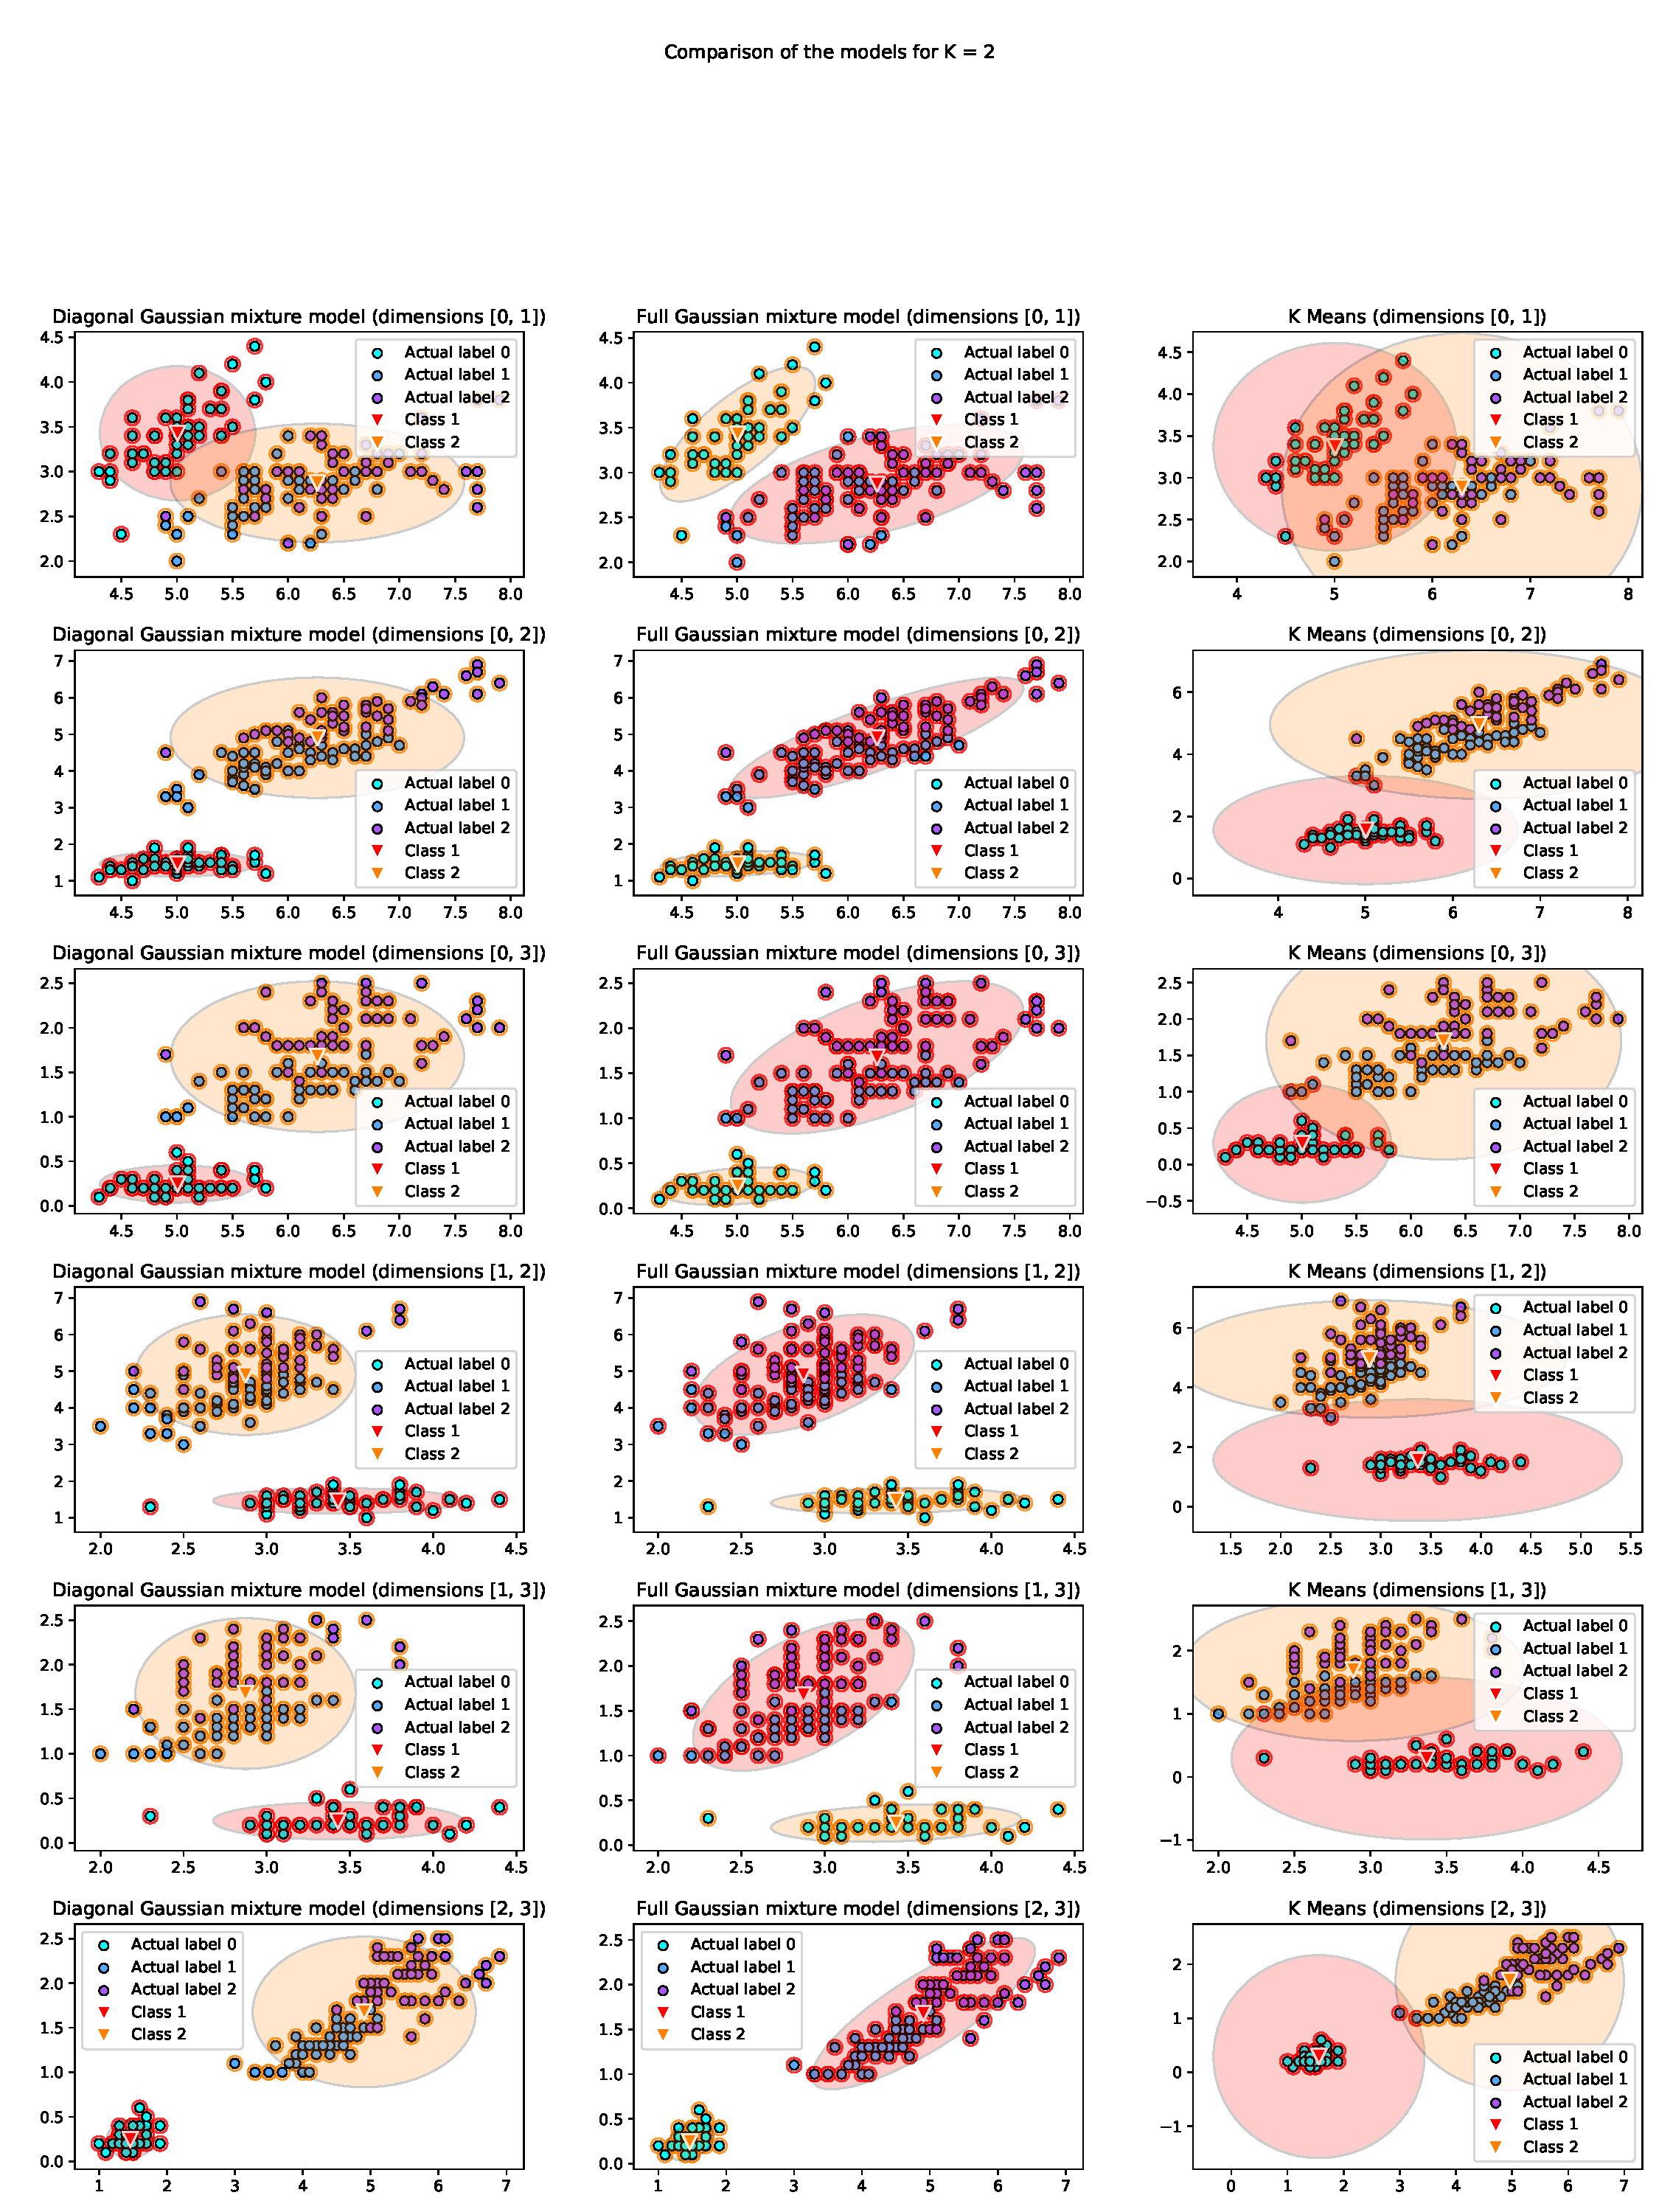
\includegraphics[width=1\textwidth]{probabilistic_graphical_models/HW2/images/iris_GM_KM_2.pdf}
            \caption{}
            \label{fig:iris2}
        \end{figure}
        
        \begin{figure}
            \centering
            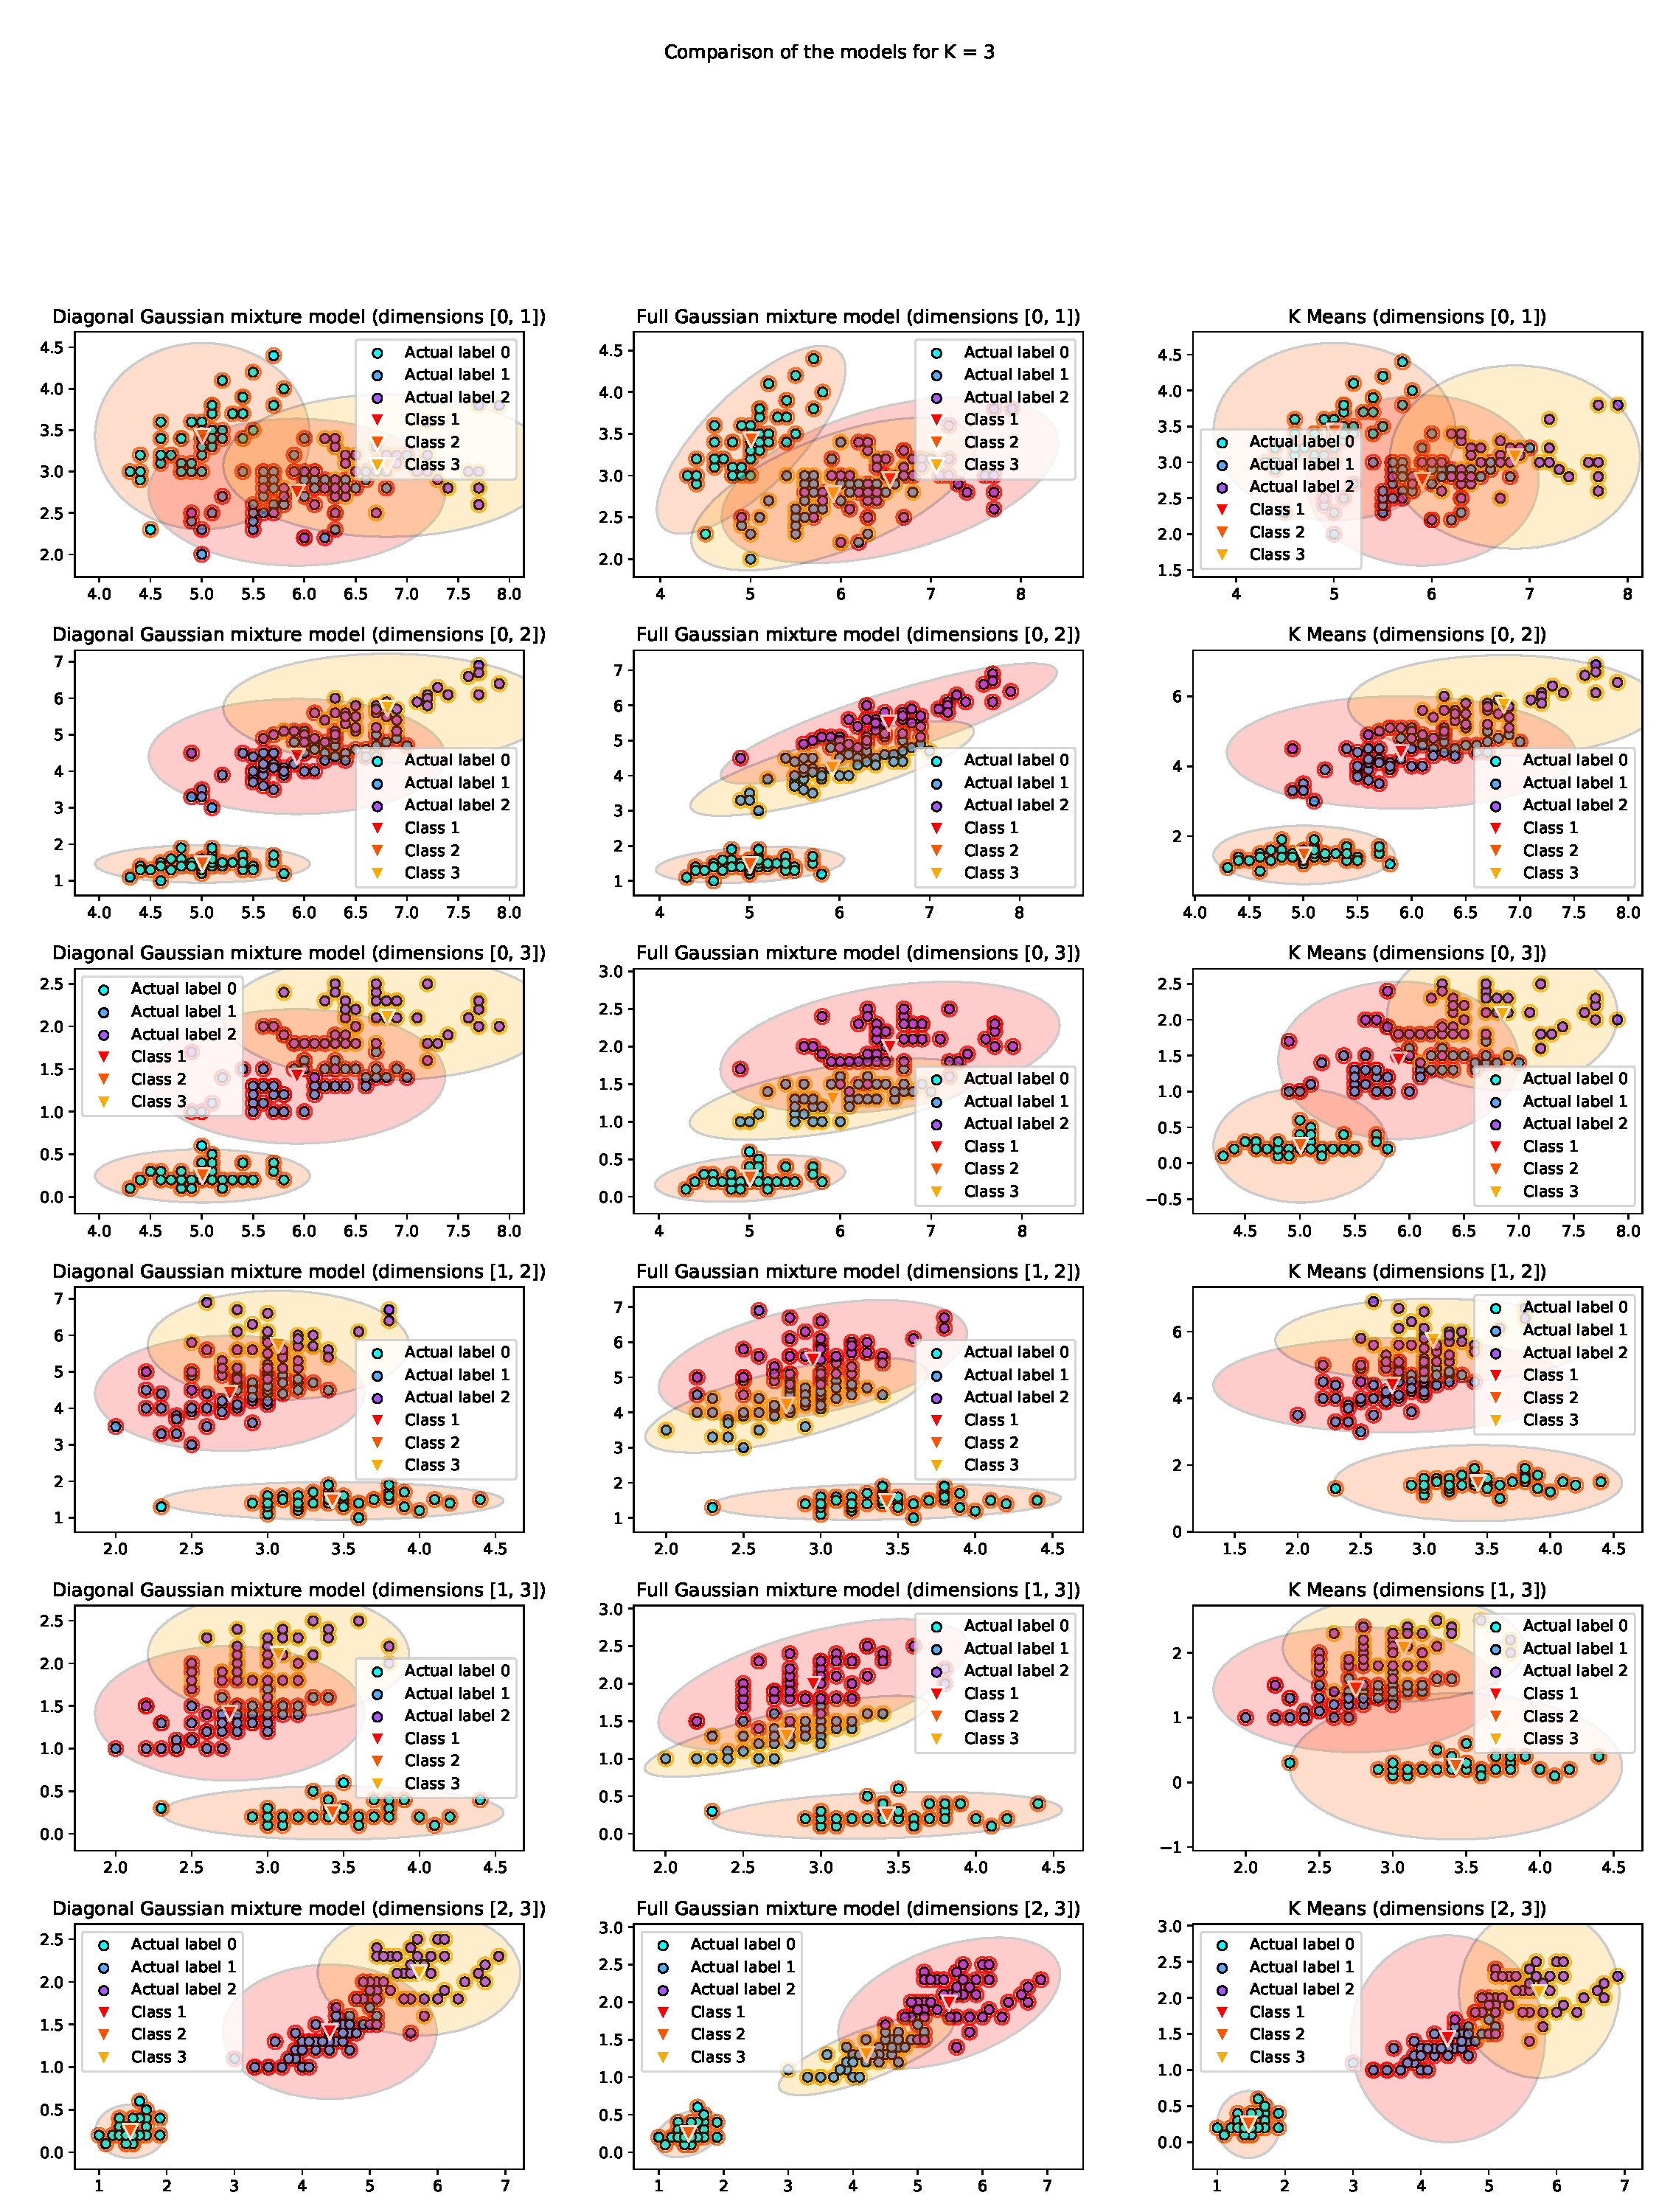
\includegraphics[width=1\textwidth]{probabilistic_graphical_models/HW2/images/iris_GM_KM_3.pdf}
            \caption{}
            \label{fig:iris3}
        \end{figure}
        
        \begin{figure}
            \centering
            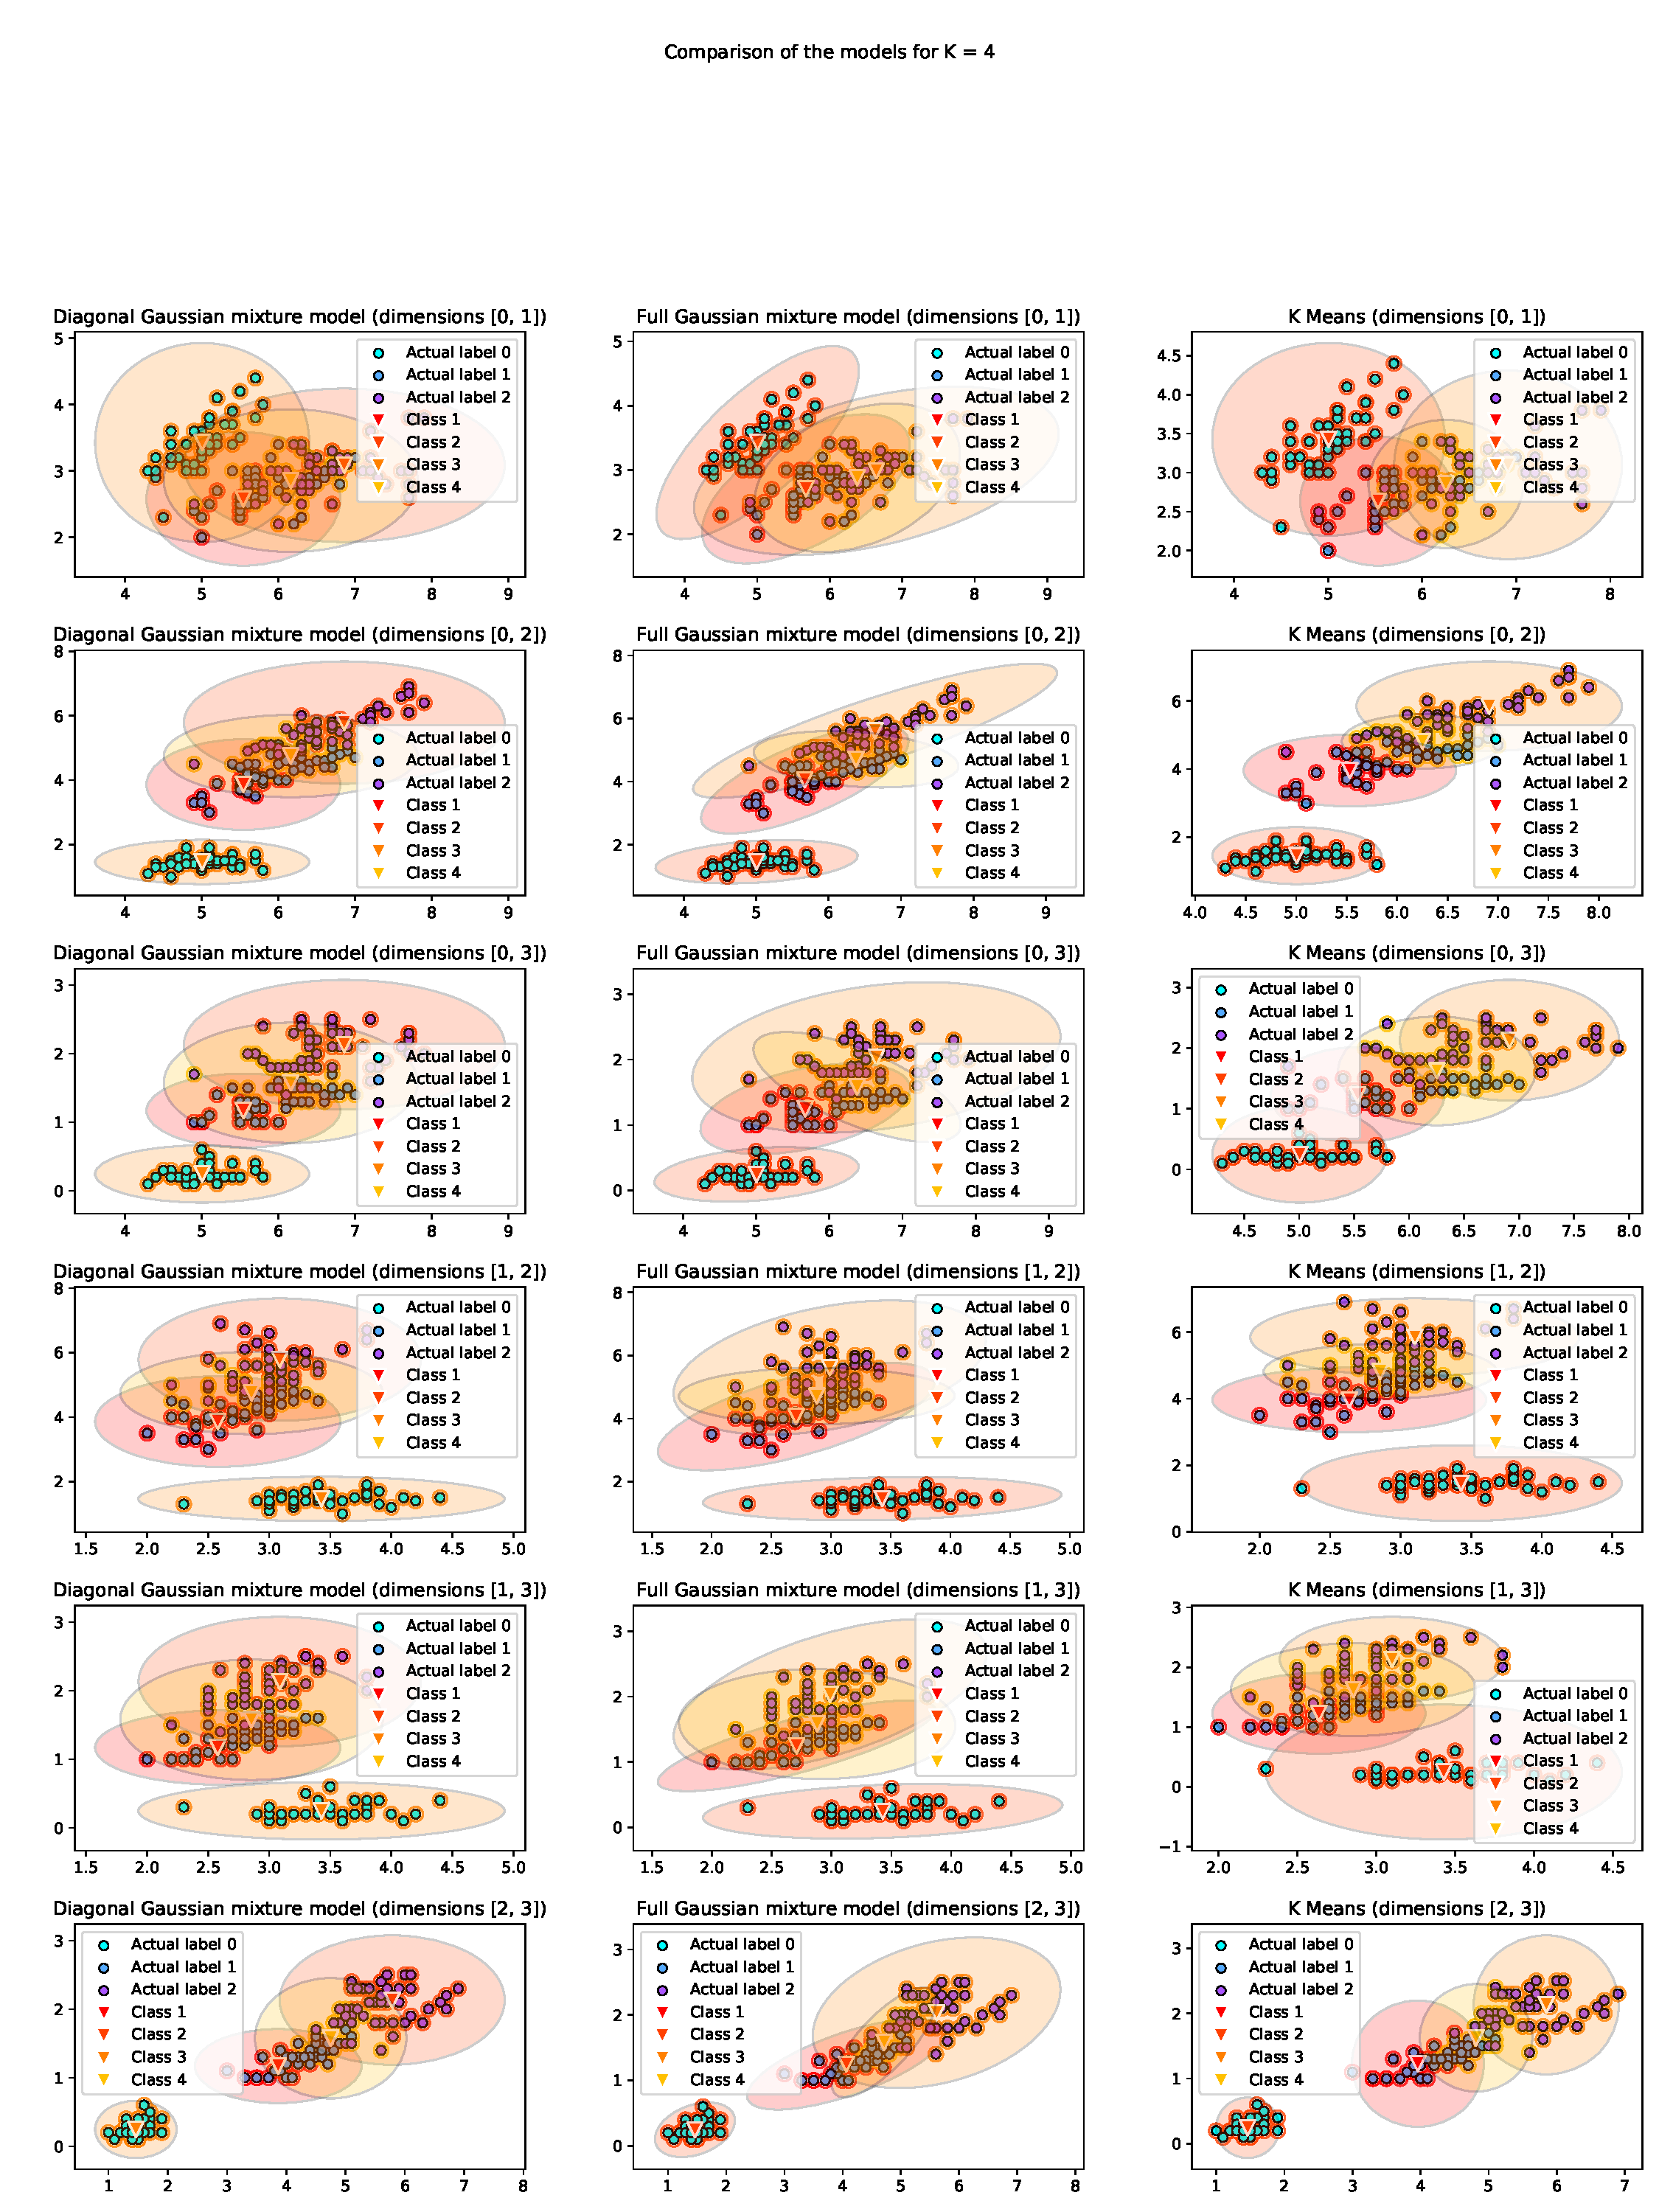
\includegraphics[width=1\textwidth]{probabilistic_graphical_models/HW2/images/iris_GM_KM_4.pdf}
            \caption{}
            \label{fig:iris4}
        \end{figure}
        
        Figures \ref{fig:iris2}-\ref{fig:iris3}-\ref{fig:iris4} , each for a specific $ K \in \{2, 3, 4\}$, are made up of six lines for each possible pair of dimensions and and three columns comparing the confidence ellipses obtained via the diagonal Gaussian Mixture model and the full Gaussian Mixture model and the spherical clusters obtained by a K Means algorithm.
        
    \item In which situations K-means is going to be significantly outperformed by the two EM algorithms discussed above? 
    
        \textbf{Solution.}\\
        \begin{figure}
            \centering
            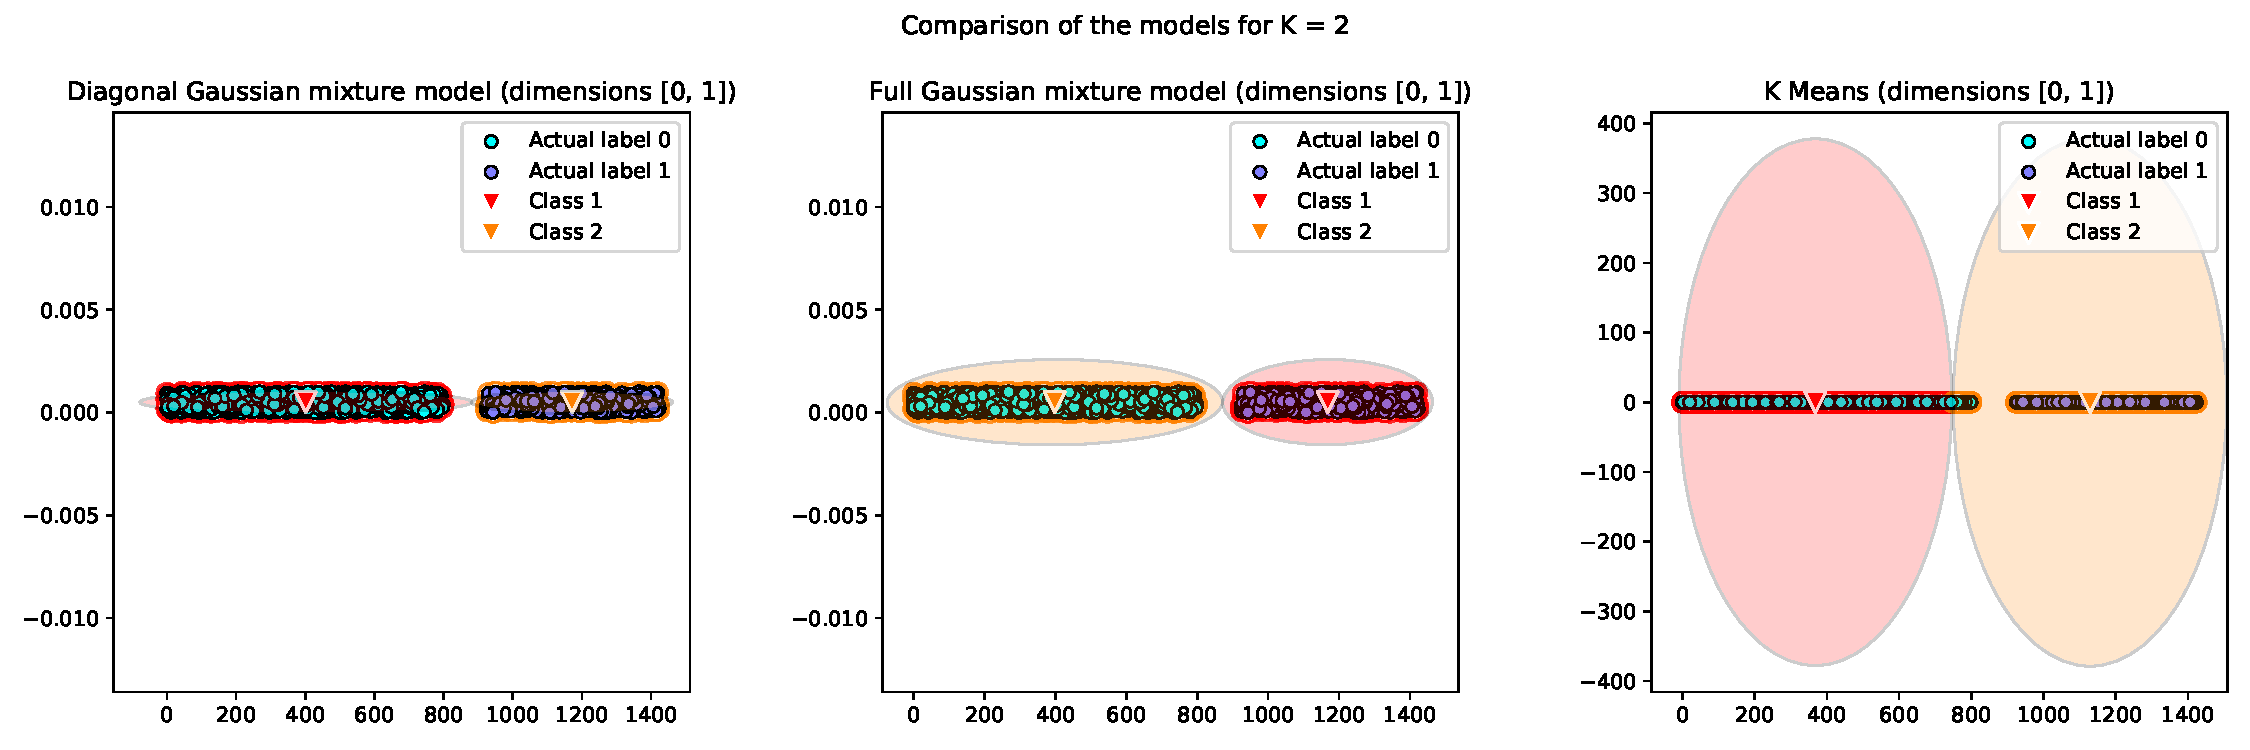
\includegraphics[width=1\textwidth]{probabilistic_graphical_models/HW2/images/custom_GM_KM_2.pdf}
            \caption{}
            \label{fig:custom1}
        \end{figure}
        
        K-means performs well when the width of the different clusters are similar, since it works by minimizing the radius of each cluster. However, K-means has a lower performance than Gaussian mixtures when the widths are quite different, as seen on figure \ref{fig:custom1}.

        \begin{figure}
            \centering
            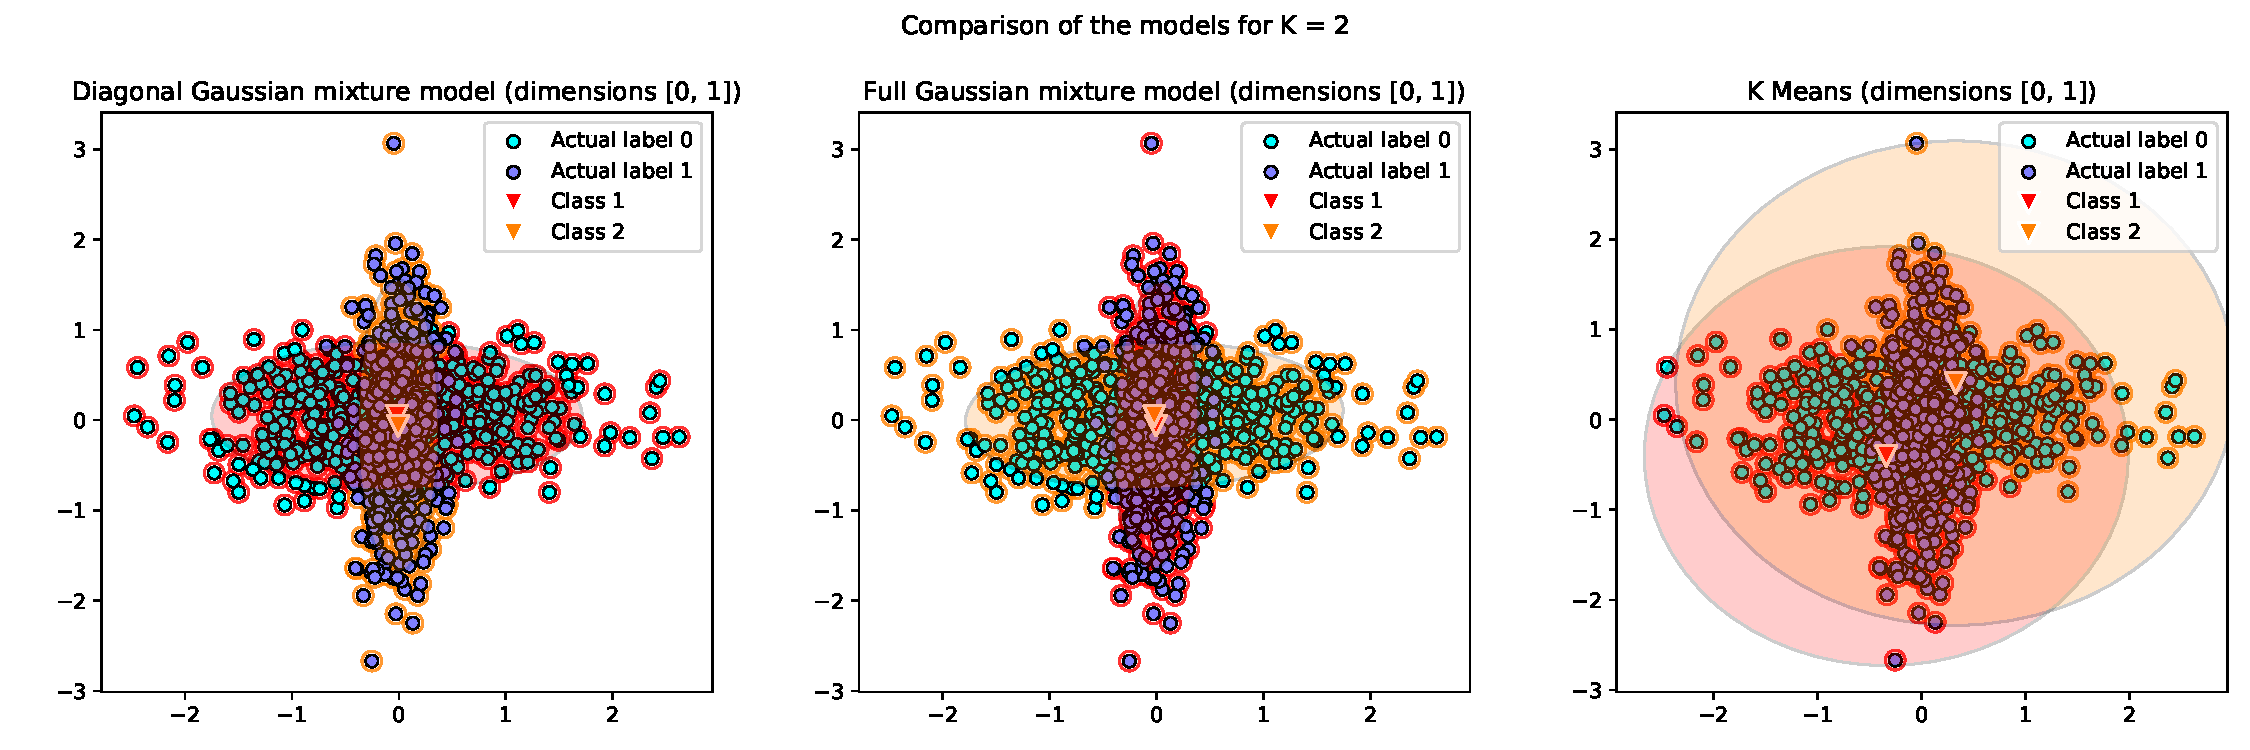
\includegraphics[width=1\textwidth]{probabilistic_graphical_models/HW2/images/custom2_GM_KM_2.pdf}
            \caption{}
            \label{fig:custom2}
        \end{figure}
        
        As well, K-means creates spheres, as opposed to the ellipses obtained with Gaussian mixtures (whether with diagonal or full covariance matrices). Therefore, Gaussian mixture models work much better than a K Means algorithm on elliptical data, as seen on figure \ref{fig:custom2}.
        

        
\end{enumerate}




\pagebreak
\chapter{Graphs, algorithms and Ising}

To avoid over or underflow, it is often recommended to store and compute small quantities (such as probabilities, densities, etc.) on the \emph{log scale}. To multiply two quantities stored on the log-scale, we just add their logs. To add two such quantities, we use the log-sum trick: if $a \geq b$, compute $\log \left( e^a + e^b \right)$ as: $a + \log \left( 1 + e^{b-a} \right)$; otherwise swap $a$ and $b$.

\begin{enumerate}
    \item Implement the sum-product algorithm for an undirected chain, using this trick, in order to compute all the forward and backward messages. (Explain how you represent the input of the algorithm, \ie, the functions $\psi_i$ and $\psi_{i, i+1}$). \\
    
    \textbf{Solution.} Let's consider $X_1, \dots, X_n$ $n$ random variables represented by an undirected chain and with joint distribution $p(x)$:

    \begin{equation*}
        p(x) = \frac{1}{Z} \prod_{i=1}^{n} \psi_i(x_i) \prod_{i=2}^{n} \psi_{i-1, i}(x_{i-1}, x_i)
    \end{equation*}
    
    Recall that the forward and backward messages can be computed with:
    
    \begin{equation*}
        \begin{aligned}
        \mu_{j \rightarrow j+1} \left( x_{j+1} \right) &= \sum_{x_j} \psi_j(x_j) \psi_{j, j+1} \left( x_j, x_{j+1} \right) \mu_{j-1 \rightarrow j} \left( x_j \right) \\
        \mu_{j \rightarrow j-1} \left( x_{j-1} \right) &= \sum_{x_j} \psi_j(x_j) \psi_{j-1, j} \left( x_{j-1}, x_j \right) \mu_{j+1 \rightarrow j} \left( x_j \right)
        \end{aligned}
    \end{equation*}
    
    Then, for $j = 1, \dots, n$, the messages can be used to compute the marginal distribution of the node $j$:
    
    \begin{equation*}
        p \left( x_j \right) &= \frac{1}{Z} \mu_{j-1 \rightarrow j} \left( x_j \right) \psi_j \left( x_j \right) \mu_{j+1 \rightarrow j} \left( x_j \right)
    \end{equation*}
    
    as well as the partition function:
    
    \begin{equation*}
        Z = \sum_{x_j} \mu_{j-1 \rightarrow j} \left( x_j \right) \psi_j \left( x_j \right) \mu_{j+1 \rightarrow j} \left( x_j \right) 
    \end{equation*}
    
    The functions $\psi_i, \psi_{i-1, i} \geq 0$ are the \emph{potentials}. In practice, they can be stored in arrays, e.g. if $X_1$ can take $K_1$ different values and $X_2$ can take $K_2$ different values, $\psi_1, \psi_2, \psi_{1, 2}$ will be stored in three arrays with shape $\left(K_1,\right), \left(K_2,\right), \left(K_1, K_2\right)$, respectively. Note that it is the same whether the random variables are discrete or continuous because in the latter case, a discretized version is used. Besides, as indicated, the log-sum trick is used for the computations. The code is available in the file \texttt{undirected\_chain.py} where an example is shown. \\
\end{enumerate}

The Ising model assumes $n$ binary variables $X_1, \dots, X_n$, which are jointly distributed as follows:

\begin{equation*}
    p \left( x_1, \dots, x_n \right) = \frac{1}{Z \left( \alpha, \beta \right)} \exp \left( \alpha \sum_{i} x_i + \beta \sum_{i \sim j} \mathbb{I}_{x_i = x_j} \right)
\end{equation*}

where the relation $i \sim j$ means that $i$ and $j$ are "neighbours". Specifically, each variable is associated to a point in a $2D$ grid, of size $h \times w$ (height times width), and two variables are neighbours if they are at distance one on that grid (\ie immediately to the left, right, up or down).

\begin{enumerate}[resume]
    \item For $w = 10, h = 100, \alpha = 0$, use your implementation from point $1$ to compute \emph{exactly} $Z \left( \alpha, \beta \right)$ as a function of $\beta$, and plot it. (Hint: recall the idea behind the junction tree algorithm).
    
    \begin{figure}
        \centering
        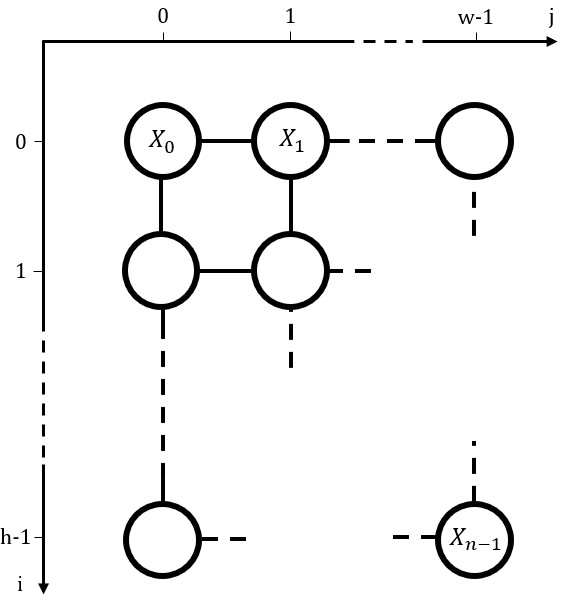
\includegraphics[scale=.7]{images/ising_model.jpg}
        \caption{Graphical model associated to the Ising model. The grid has a size $h \times w$ and contains $n = h \times w$ vertices.}
        \label{fig:ising}
    \end{figure}
    
    \textbf{Solution}. The graph $G = \left( V, E \right)$ corresponding to the Ising model is represented in figure \ref{fig:ising}. For simplicity and to fit with the code, the indices are translated from $[\![ 1, n ]\!]$ to $[\![ 0, n-1 ]\!]$. Let $k \in [\![ 0, n-1 ]\!]$. There exists a pair $(i, j) \in [\![ 0, h-1 ]\!] \times [\![ 0, w-1 ]\!]$ such that $k = i \times w + j$. The node associated to $X_k$ can be denoted by $v_{i, j}$ and corresponds to the node at the $i$-th row and the $j$-column. The idea here is to turn every row into a super-node to retrieve the case of the question $1$ with an undirected chain that contains $h$ nodes who can take $2^{w}$ different states. This choice comes from the fact that $w = 10 < 100 = h$ and this is more efficient to have $2^{10}$ possible states rather than $2^{100}$. Let's rewrite the joint distribution:
    
    \begin{equation*}
        \begin{aligned}
        p \left( x_0, \dots, x_{n-1} \right) &= \frac{1}{Z \left( \alpha, \beta \right)} \exp \left( \alpha \sum_{k=0}^{n-1} x_k + \beta \sum_{k \sim l} \mathbb{I}_{x_k = x_l} \right) \\
        &= \frac{1}{Z \left( \alpha, \beta \right)} \left( \prod_{k=0}^{n-1} e^{\alpha x_k} \right) \left( \prod_{k \sim l} e^{\beta \mathbb{I}_{x_k = x_l}} \right) \\
        &= \frac{1}{Z \left( \alpha, \beta \right)} \left( \prod_{i=0}^{h-1} \prod_{j=0}^{w-1} e^{\alpha v_{i, j}} \right) \left( \underbrace{\prod_{i=0}^{h-1} \prod_{j=0}^{w-2} e^{\beta \mathbb{I}_{v_{i, j} = v_{i, j+1}}}}_{\text{horizontal edges}} \underbrace{\prod_{i=0}^{h-2} \prod_{j=0}^{w-1} e^{\beta \mathbb{I}_{v_{i, j} = v_{i+1, j}}}}_{\text{vertical edges}} \right) \\
        &= \frac{1}{Z \left( \alpha, \beta \right)} \prod_{i=0}^{h-1} \left( \prod_{j=0}^{w-1} e^{\alpha v_{i, j}} \prod_{j=0}^{w-2} e^{\beta \mathbb{I}_{v_{i, j} = v_{i, j+1}}} \right) \prod_{i=0}^{h-2} \left( \prod_{j=0}^{w-1} e^{\beta \mathbb{I}_{v_{i, j} = v_{i+1, j}}} \right) \\
        &= \frac{1}{Z \left( \alpha, \beta \right)} \prod_{i=0}^{h-1} \phi_{i} \left( x_{R_i} \right) \prod_{i=0}^{h-2} \phi_{i, i+1} \left( x_{R_i}, x_{R_{i+1}} \right) \\
        &\triangleq \Tilde{p} \left( x_{R_0}, \dots, x_{R_{h-1}} \right)
        \end{aligned}
    \end{equation*}

    where $R_i$ is just the $i$-th, i.e. the set of nodes $\left\{ v_{i, j} \right\}_{j \in [\![ 0, w-1 ]\!]}$. Hence, it is possible to use the undirected chain formed by the super-nodes $x_{R_0}, \dots, x_{R_{h-1}}$ to compute $Z \left( \alpha, \beta \right)$. The result is shown in figure \ref{fig:log-partition}, with $\beta \in [-2, 2]$. This can be obtained by running the file \texttt{ising.py}, which contains both the class \texttt{Ising} and a small script to plot the log-partition function.
    
    \begin{figure}
        \centering
        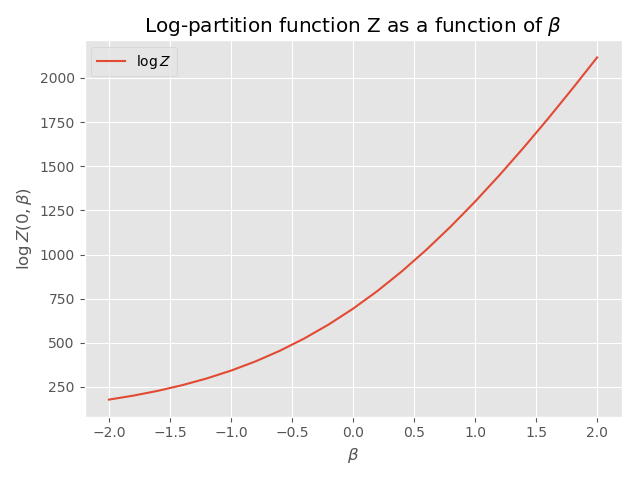
\includegraphics[scale=.5]{images/log_partition_beta.png}
        \caption{Log-partition function as a function of $\beta$ and with $\alpha = 0$.}
        \label{fig:log-partition}
    \end{figure}
    
    \item Implement loopy belief propagation to obtain a faster approximation of $Z \left( \alpha, \beta \right)$. (Explain.) For which values of $\beta$ the approximation error gets larger?
    
    \textbf{Solution}. The implementation of the loopy belief propagation algorithm is available in the file \texttt{loopy\_belief\_propagation.py}. For each node, we send a message to its neighbors using the following formula and we iterate:
    
    \begin{equation*}
        \mu_{i \rightarrow j} \left( x_j \right) = \sum_{x_i} \psi_i \left( x_i \right) \psi_{i, j} \left( x_i, x_j \right) \prod_{k \in \mathcal{N} \left( i \right) \setminus \left\{ j \right\}} \mu_{k \rightarrow i} \left( x_i \right)
    \end{equation*}
    
    \begin{figure}[h]
        \centering
        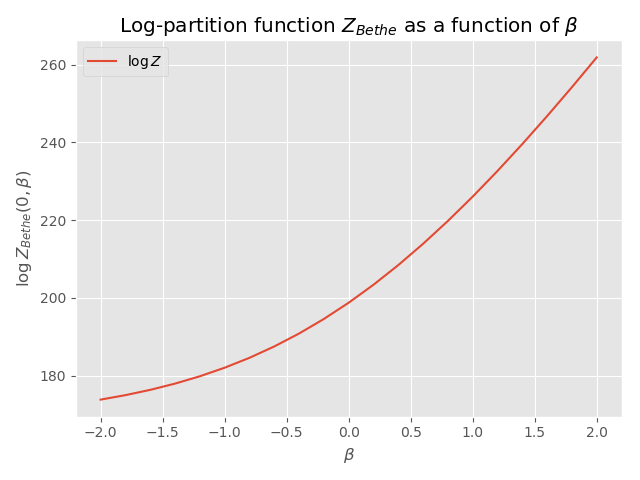
\includegraphics[scale=.5]{images/approx_log_partition_beta.png}
        \caption{Approximation of the log-partition function as a function of $\beta$.}
        \label{fig:approx-log-partition}
    \end{figure}
    
    The result for ten passes is shown in figure \ref{fig:approx-log-partition}. We see that it is very similar to the result obtained in the previous question, except that the values are different. Besides, the log-partition function obtained now depends on both the marginal used and the number of passes. For instance, with the top-left corner node and after $5$ passes, the marginal is computed using the information of $15$ nodes, where as with the node indexed by $(5, 5)$, $61$ nodes are used. It corresponds to the $5$-order neighborhood of the two nodes, respectively.
    
    We see that when $\beta$ is small, the difference between the two functions is small, and vice-versa. We do not really know what is expected here and it is not fully detailed in the lecture notes, but in the literature, it is possible to find some formulas computing the quantity $\frac{Z}{Z_{Bethe}}$, where $Z_{Bethe}$ is the Bethe approximation obtained with the loopy belief algorithm. This quantity involves the so-called "beliefs" terms.
\end{enumerate}

\end{document}
